\section{Sensor space analysis}
An important step in analyzing data at single-subject and group levels is sensor-space analysis. Here we show how several different techniques can be employed to understand the data.

\begin{figure}[t]
  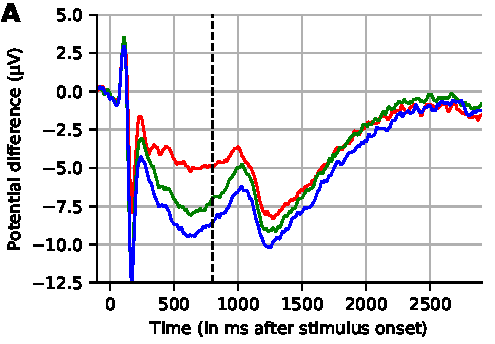
\includegraphics[width=0.49\linewidth]{figures/grand_average_highpass-NoneHz.pdf}
  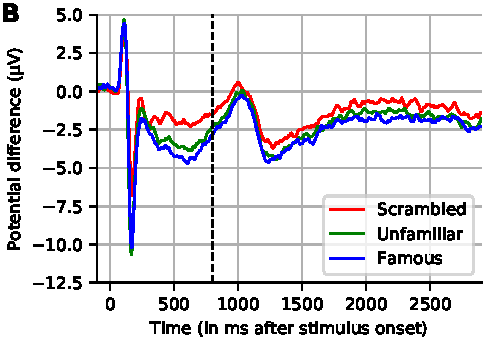
\includegraphics[width=0.49\linewidth]{figures/grand_average_highpass-1Hz.pdf}
\caption[Grand averaged evoked response across 16 subjects.]{Grand averaged evoked response across 16 subjects for channel EEG065.
(A) No highpass filter. (B) Highpass filtered at 1.0 Hz. Note that, similar to (A), the results reported by \cite{wakeman2015multi} (dashed line at 800 ms indicates where their plot stopped) show large drifts, but these return to near-baseline levels toward the end of a sufficiently long interval (here, 2.9 seconds) even without applying a highpass filter.}
\label{fig:grand_average}
\end{figure}  

\subsection{Group average}

A classical step in group studies is known as ``grand averaging''~\citep{delorme-etal:15}. It is particularly common for EEG studies and it consists in averaging ERPs across all subjects in the study. As not all subjects have generally the same good channels, this step is commonly preceded by an interpolation step to make sure data are available for all channels and for all subjects. Note that grand averaging is more common for EEG than for MEG, as MEG tends to produce more spatially resolved topographies that may not survive averaging due to signal cancellations.

The grand average of the 16 subjects for one EEG sensor (EEG065) is presented in Figure~\ref{fig:grand_average}. We selected this channel to compare with the figure proposed by \cite{wakeman2015multi}. We present the grand average for the `scrambled', `famous', and `unfamiliar' conditions using a high-pass filter (cf. Section~\ref{sec:baseline}), and baseline corrected using prestimulus data. This figure replicates the results in \citep{wakeman2015multi}. We can see the early difference between faces, familiar or unfamiliar, and scrambled faces around 170\,ms. We can also notice a difference in the late responses between the two conditions `unfamiliar' and `famous'. However, the effect is smaller when using high-pass filtering, as it corrects for the slow drifts.

\emph{Caveats} For MEG, the grand average may wash out effects or induce spurious patterns due to misalignment between head positions. SSS can be used to align subjects in one common coordinate systems.
    
\subsection{Contrasting conditions}

Two conditions of interest are often compared using a statistical contrast. A paired contrast between two conditions can be computed by computing the difference in their evoked responses. The difference does not take into account the number of trials used to compute the evoked response -- in other words, each condition is weighted equally. Recall that the event IDs were organized hierarchically during epoching (as described in Section~\ref{sec:epoching}). Such a hierarchical organization is natural for contrasting conditions in the experiment, as we compare not only `faces' against `scrambled faces', but also `famous faces' against `unfamiliar faces'.
    
\emph{Caveats.} Although this is standard in EEG pipelines, historically, for computing the source estimates, weighted averages have sometimes been used. However, MNE provides a mathematically correct estimate for the effective number of trials averaged, so equal-weighted combinations (additions or subtractions) of evoked data are properly accounted for even in the context of unequal trial counts. This logic, however, does not apply when working with experimental protocols (for example, oddball tasks) which, by design, produce many more examples of one than the other conditions.

\subsection{Cluster statistics}

\begin{figure}
\centering
    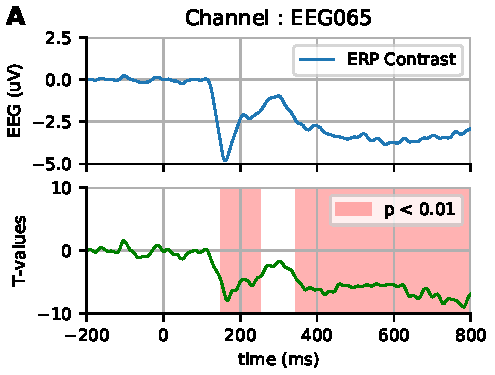
\includegraphics[width=0.49\linewidth]{figures/sensorstat_highpass-NoneHz.pdf}
    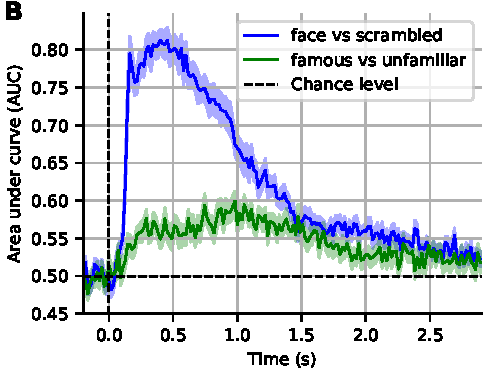
\includegraphics[width=0.49\linewidth]{figures/time_decoding_highpass-NoneHz.pdf}
    \caption[Sensor space statistics.]{Sensor space statistics. (A) A single sensor (EEG065) with temporal clustering statistics. The clustering is based on selecting consecutive time samples that have exceeded the initial paired t-test threshold (0.001), and finding clusters that exceed the size expected by chance according to exchangeability under the null hypothesis ($p < 0.01$, shaded areas). (B) AUC score of time-by-time decoding, averaged across cross validation folds. As opposed to a cluster statistic, time decoding is a multivariate method which pools together the signal from different sensors to find discriminative time points between two conditions.}
\label{fig:fig_sensorstat}
\end{figure}

To contrast our conditions of interest, here we use a non-parametric clustering statistical procedure as described by \cite{maris_nonparametric_2007}. This combines neighboring values that are likely to be correlated (here, neighboring time instants) to reduce the problem of multiple comparisons. The contrast score (here the  t-values) for each cluster are summed up to compute the mass of each cluster, which serves as our actual statistic. Next, we need to know if the distribution data in our two conditions (here measured using cluster sizes) is significantly different from what would be obtained by chance. For this purpose, we generate a null distribution from the data by randomly swapping our conditions for each subject according to exchangeability under our null hypothesis. In this case, it is equivalent to changing the sign of the contrast data (as we are using a one-sample t-test on the difference between conditions), and then recomputing the maximal cluster size for each permutation. From an estimate of the distribution of the maximum cluster size under the null-hypothesis, we can compute the probability of observing each cluster relative to this distribution. This gives us a control of the type I error, when reporting a significant difference between the distribution of data in our two conditions.

Running this nonparametric permutation test on the single sensor EEG065 (also used by \cite{wakeman2015multi}) revealed two across-time clusters that allowed us to reject the null hypothesis at the level $p < 0.01$. To perform the clustering, we used an initial thresholding of $p < 0.001$ with a two-sided paired t-test (Figure~\ref{fig:fig_sensorstat}). The statistic used was a one-sample t-test on the contrast ERPs using as contrast weights (0.5 for 'familiar', 0.5 for 'unfamiliar' and -1 for 'scrambled'), testing for the condition faces versus scrambled faces. A first cluster appears around the same time as the evoked response, and the other captures the late effects. Running another statistical test, this time incorporating the spatial distribution of the sensors into the clustering procedure, yields one spatiotemporal cluster with $p < 0.05$ for the contrast condition as shown in Figure~\ref{fig:stclusterstats}.

\begin{figure}
\centering
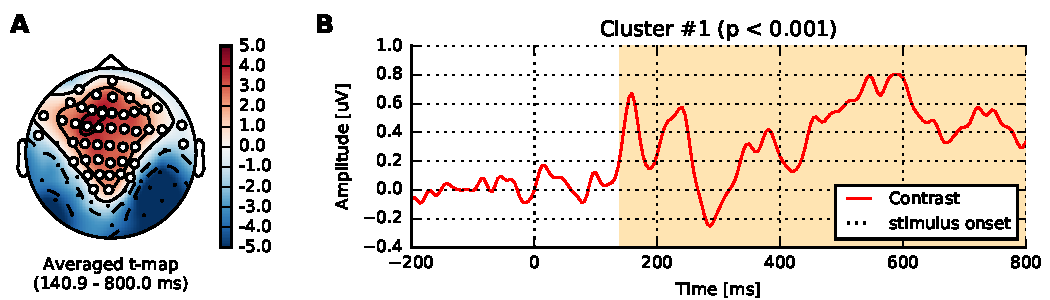
\includegraphics[width=\linewidth]{figures/spatiotemporal_stats_cluster_highpass-NoneHz-00.pdf}
\caption[Spatiotemporal cluster statistics on EEG sensors.]{Spatiotemporal cluster statistics on the EEG sensors. (A) Topographic map of the t-statistic. (B) Average over the sensors that were part of the significant cluster.}
\label{fig:stclusterstats}
\end{figure}
\emph{Alternatives and caveats.} It is important to note that this clustering permutation test does not provide feature-wise (vertex, sensor, time point, etc.) but \emph{cluster-level} inference. This is because the test statistic is the cluster size and not any specific t-values used to obtain the cluster in the first place. When inspecting a significant cluster, no conclusion can be drawn on which time point or location was more important. A computationally more expensive alternative is the so-called TFCE method which provides feature-level inference and, moreover, mitigates the problem of having to set the initial threshold on the t-values to define clusters~\citep{TFCE}. When strong \emph{a priori} hypotheses exist considering few regions of interest in either time, frequency or space can be a viable alternative. In that case, the multiple comparisons problem may be readily alleviated by more conventional measures, such as \acp{FDR} \citep{FDR}.

\subsection{Time Decoding}

As an alternative to mass-univariate analysis, a event-related brain dynamics can studied using a multivariate decoding approach~\citep{ramkumar2013feature,king2014characterizing}. Here, a pattern classifier, often a linear model (e.g. logistic regression) is trained to discriminate between two conditions: `face' versus `scrambled', and also `famous faces' versus `unfamiliar faces'. The classifier can be trained on single trials, time-point by time-point. The prediction success can then be assessed with cross-validation at every instant, yielding an intuitive display of the temporal evolution of discrimination success. In Figure~\ref{fig:fig_sensorstat}B, we display such cross-validation time-series averaged across the 16 subjects. As anticipated, discriminating between faces and scrambled faces is much easier than discriminating between `famous' and `unfamiliar' faces, based on information in early components in the first second after stimulus-onset.

For performance evaluation, we use is area under the receiver operating characteristic curve (ROC-AUC), as it is a metric that is insensitive to class imbalance (i.e., differing numbers of trials) therefore allowing us to average across subjects, and also to compare the two classification problems (faces vs. scrambled and familiar vs. unfamiliar). Results on the faces vs. scrambled conditions show that time-resolved decoding reveals decoding accuracy greater than chance around the same time intervals as the non-parametric cluster statistic. The effect although appears here quite sustained over time. Results on familiar \emph{vs.} unfamiliar conditions are also above chance from 200 to 300\,ms, however the best decoding performance emerges later for this contrast. This more subtle effect even peaks after 800\,ms, which exceeds the time window investigated in the original study.
